\chapter*{\textsl{Liminaire}}
\phantomsection

\addcontentsline{toc}{chapter}{\textsl{Liminaire}}
\thispagestyle{empty}

\bigskip

With the advent of the internet, sharing and access knowledge have opened a new world of communication toward I hope a new real world. Here is my contribution as a composer of what I call `conceptual music'.						
\bigskip

Conceptual Music consists to highlight and formulate a nodal point of acquired concepts that can be understood in ontological terms. In essence, a concept is the formalisation of structuring object(s) whose emerging phenomenology is either deterministic or indeterministic, and identified as such. My purpose is to point out some nodal points notably through the programming language paradigm as for instance a sketch, a description or a process. This is naturally a work in progress, and the philosophical interpretation of the concept as such remains to be done.						

Or, to put it another way, the definition of the concept in a musical context, consists to pin down the emergent phenomenon as a nodal point of structuring elements. The emergent phenomenon is the sonic object itself that I produce to questioning or integrating my environment as a significative nodal point.

\bigskip
 
The application -- as performances or as scores for instance -- of the said concepts aim to stimulate the imagination and possibly even the creativity of the listener, notably by anamnesis in cognitive terms.										

\bigskip

\begin{center}\rule{0.5\linewidth}{0.5pt}\end{center}

\bigskip
\bigskip

\textbf{Note}: Some codes are stamped \texttt{\textcolor{red}{\small[private]}} because they are too messy to be shared. They will be re-writed and rationalised to be so.
%\newpage

\chapter*{Works}
\phantomsection

\addcontentsline{toc}{chapter}{Works}

\section*{Ghost Wind}
\phantomsection

\addcontentsline{toc}{section}{Ghost Wind}
\thispagestyle{empty}

\bigskip

\begin{description}
\item[Concept] \hfill 
\begin{itemize}
\item[] Wind synthesis correlated to a spoken word recording using pitch analysis and formantic analysis with a degree of shape smoothing.
\end{itemize}
\bigskip
\item[Context] \hfill 
\begin{itemize}
\item[] Study in the framework of the acousmatic tale \textit{The Robot And The Baby} conducted by Fr\'{e}d\'{e}ric Voisin in 2012. \\
$\rightarrow$ \href{http://www.fredvoisin.com/spip.php?article215}{\texttt{\small http://www.fredvoisin.com/spip.php?article215}}
\end{itemize}
\bigskip
\item[Required] \hfill 
\begin{itemize}
\setlength\itemsep{1em}
\item[] \texttt{BASH} \\ $\rightarrow$ \href{https://www.gnu.org/software/bash}{\texttt{\small https://www.gnu.org/software/bash}}
\item[] \texttt{PRAAT} \\ $\rightarrow$ \href{http://www.fon.hum.uva.nl/praat}{\texttt{\small http://www.fon.hum.uva.nl/praat}} 
\item[] \texttt{SBCL} \\ $\rightarrow$ \href{http://www.sbcl.org}{\texttt{\small http://www.sbcl.org}}
\end{itemize}
\bigskip
\item[Source] \hfill 
\begin{itemize}
\item[] $\rightarrow$ \href{https://github.com/yannics/GSA/SC/ghost-wind}{\texttt{\small https://github.com/yannics/GSA/SC/ghost-wind}} -- \texttt{\textcolor{red}{\small[private]}}
\end{itemize}
\bigskip
\newpage
\setcounter{footnote}{0}
\item[Alternative] \hfill 
\begin{itemize}
\item[] The \textsl{UGen} \texttt{LPCAnalyzer} with noise as the source -- sounding windy in that way -- uses the linear predictive coding analysis
\citep{mak} %\footnote{\setstretch{0.8}John Makhoul. \textit{Linear Prediction: A Tutorial Review}. Proceedings of the IEEE 63(4), 1975. \\ \href{http://www.ee.iitm.ac.in/~giri/pdfs/reading\_material/Markhoul.pdf}{\scriptsize{\texttt{http://www.ee.iitm.ac.in/$\sim$giri/pdfs/reading\_material/Markhoul.pdf}}} \normalsize{}}
on the input signal, but in this case, the formantic part is eluded because it works only as frequency bandwidths of which the size is determined by the parameter \texttt{noise}. 

\smallskip

\begin{lstlisting}
SynthDef(\LPC, {
  | outBus=0, inBus=0, amp=0, noise=256, 
    xpos=0, ypos=0 |
  Out.ar(outBus, 
    Pan4.ar(
      LPCAnalyzer.ar(
        In.ar(inBus, 1), 
        PinkNoise.ar(0.25), 
        1024, 
        noise), 
      xpos, ypos, amp))
}).add;
\end{lstlisting}
\end{itemize}
\end{description}

\bigskip

\begin{center}\rule{0.5\linewidth}{0.5pt}\end{center}

\bigskip

\section*{\texttt{RM236}}
\phantomsection

\addcontentsline{toc}{section}{\texttt{RM236}}

\bigskip

\begin{description}
\item[Concept] \hfill 
\begin{itemize}
\item[] Rhythmic counterpoint -- between 5 complementary rhythms -- for 4 voices and 3 layers, with one as tuning radio sound effects, one as far low bass drums and some kind of high frequencies `sparkles'.
\end{itemize}
\bigskip
\item[Context] \hfill 
\begin{itemize}
\item[] Participation of the \textit{Lake Radio} open call -- \texttt{Works for Radio \#4} -- in 2020. \\
$\rightarrow$ \href{http://thelakeradio.com/call}{\texttt{\small http://thelakeradio.com/call}}
\end{itemize}
\bigskip
\bigskip
\item[Source] \hfill 
\begin{itemize}
\item[] $\rightarrow$ \href{https://github.com/yannics/GSA/SC/RM236}{\texttt{\small https://github.com/yannics/GSA/SC/RM236}}  -- \texttt{\textcolor{red}{\small[private]}}
\end{itemize}
\end{description}

\bigskip

\begin{center}\rule{0.5\linewidth}{0.5pt}\end{center}

\bigskip

\section*{\textsl{Selenes Havbrev}}
\phantomsection

\addcontentsline{toc}{section}{\textsl{Selenes Havbrev}}

\bigskip

\begin{description}
\item[Concept] \hfill 
\begin{itemize}
\item[] Interactive quadraphonic soundscape using Open Sound Control over WIFI with the modular control surface TouchOSC.
\end{itemize}

\item[Context] \hfill 
\begin{itemize}
\item[] 
See booklet \textsl{Bl\aa stjernehav Familie- \& Dukketeater} on page \pageref{psh}.\\
See also article in \textsl{HAKAPIC, et nettmagasin for kunstkritikk}.\\
$\rightarrow$ \href{https://www.hakapik.no/home/2020/10/8/levende-kunst-i-en-bygning-i-forfall}{\texttt{\scriptsize https://www.hakapik.no/home/2020/10/8/levende-kunst-i-en-bygning-i-forfall}}

\end{itemize}

\item[Required] \hfill 
\begin{itemize}
\setlength\itemsep{1em}
\item[] \texttt{FFmpeg} \\ $\rightarrow$ \href{https://ffmpeg.org/}{\texttt{\small https://ffmpeg.org/}}
\item[] \texttt{SOX} \\ $\rightarrow$ \href{http://sox.sourceforge.net/}{\texttt{\small http://sox.sourceforge.net}}
\item[] \texttt{TouchOSC} \\ $\rightarrow$ \href{https://hexler.net/products/touchosc}{\texttt{\small https://hexler.net/products/touchosc}}
\end{itemize}

\item[Source] \hfill 
\begin{itemize}
\item[] $\rightarrow$ \href{https://github.com/yannics/GSA/SC/SelenesHavbrev}{\texttt{\small https://github.com/yannics/GSA/SC/SelenesHavbrev}}  -- \texttt{\textcolor{red}{\small[private]}}
\end{itemize}

\item[Notes] \hfill 
\label{mp:msxy}
\begin{enumerate}
\item Quadraphonic XY/MS\\
The recording of the soundscapes is done with the recorder Zoom H2N, which allows to record in 4 channels mode, generating two stereo sound files involving respectively the microphones MS and XY.
 \begin{figure}[H]
\begin{center}
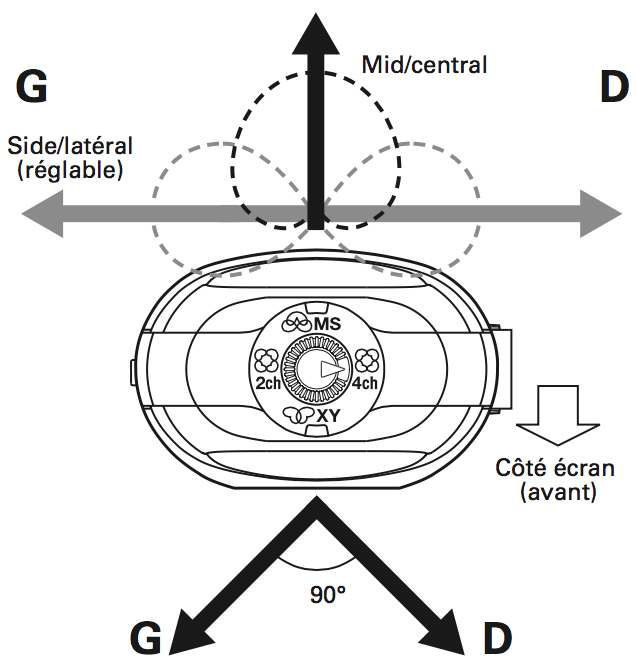
\includegraphics[scale=0.23]{mp/img/H2N.png}
%\caption{Figure on page 21 of the operational manual.}
%\label{h2n}
\end{center}
\end{figure}
\item Decode MS\\
\begin{figure}[!hbt]
	\begin{center}
		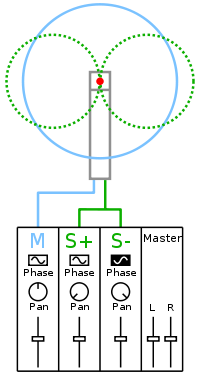
\includegraphics[width=33mm]{mp/img/MS}
	\end{center}
\end{figure}\\
\textit{D'origine allemande, MS signifie} \textsl{Mitte Seite} \textit{en Allemand et} \textsl{Middle-Side} \textit{en Anglais.
La radio st\'{e}r\'{e}ophonique transmet le signal sous la forme d'un signal monophonique, et d'un signal de diff\'{e}rence entre canaux, qui s'ajoute \`{a} gauche et se retranche \`{a} droite. La prise de son MS utilise le m\^{e}me principe d\`{e}s la captation. Une capsule cardio\"{i}de ou omnidirectionnelle est point\'{e}e vers le centre de la sc\`{e}ne sonore, une deuxi\`{e}me capsule, \`{a} directivit\'{e} en 8, est plac\'{e} perpendiculairement aussi pr\`{e}s de la premi\`{e}re que possible,
Le passage des canaux gauche et droite aux canaux M et S, et inversement, s'effectue par un proc\'{e}d\'{e} de somme et diff\'{e}rences dit matri\c{c}age:}\\ \\
$M = L + R$\\
$S = L - R$\\
$M + S = ( L + R ) + ( L - R ) = 2L$\\
$M - S = ( L + R ) - ( L - R ) = 2R$\\ \\
\textit{La profondeur de l'effet st\'{e}r\'{e}o se r\`{e}gle facilement en ajustant l'intensit\'{e} relative des deux composantes.}\footnote{\setstretch{0.8}Captation st\'{e}r\'{e}ophonique. \textit{Wikip\'{e}dia, l'encyclop\'{e}die libre.} [Page consult\'{e}e le 31/07/20]\\ \indent \href{http://fr.wikipedia.org/w/index.php?title=Captation\_st\%C3\%A9r\%C3\%A9ophonique}{\scriptsize{\texttt{http://fr.wikipedia.org/w/index.php?title=Captation\_st\%C3\%A9r\%C3\%A9ophonique}}} \normalsize{}}\\
%Manipulating audio
\item Extract audio from MP4\\
\texttt{\scriptsize \$ ffmpeg -i in.mp4 out.wav}
\item Trim audio files\\ 
\texttt{\scriptsize \$ sox initial.wav snippet.wav trim [SECOND TO START] [SECONDS DURATION]}
\item Remove part in audio files\\ 
\texttt{\scriptsize \$ sox in.wav out.wav trim 0 =[SECOND TO START] =[SECOND TO STOP]}
\item TouchOSC setup\\ 
Set iPad TouchOSC \textsf{Layout editor hosts} and \textsf{connections OSC} with the IP of the remote laptop (see \textsf{Network System Preferences}).
\begin{figure}[H]
\hfill 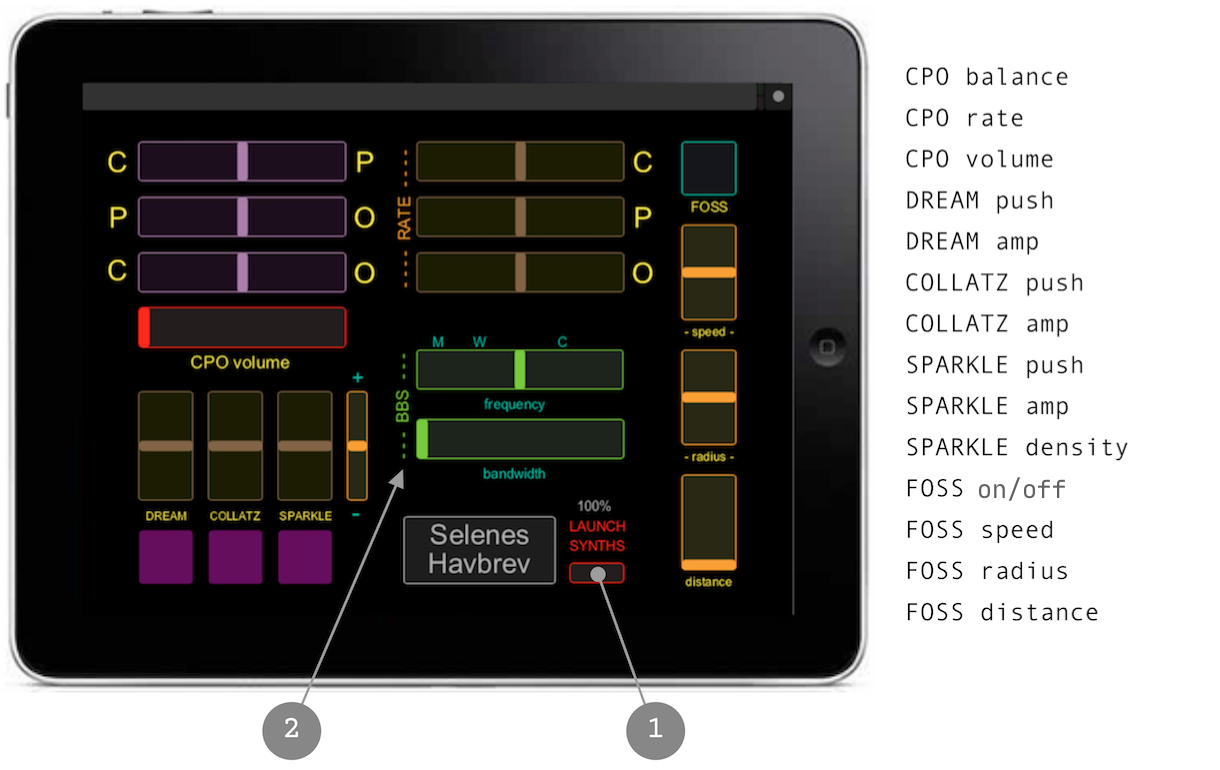
\includegraphics[width=0.87\textwidth]{mp/img/ipad1}
\end{figure}
\vspace{-5mm}
Layout used during the play on the 23rd of August 2020 at Troms\o{} Kunstforening.
\begin{figure}[H]
\hfill 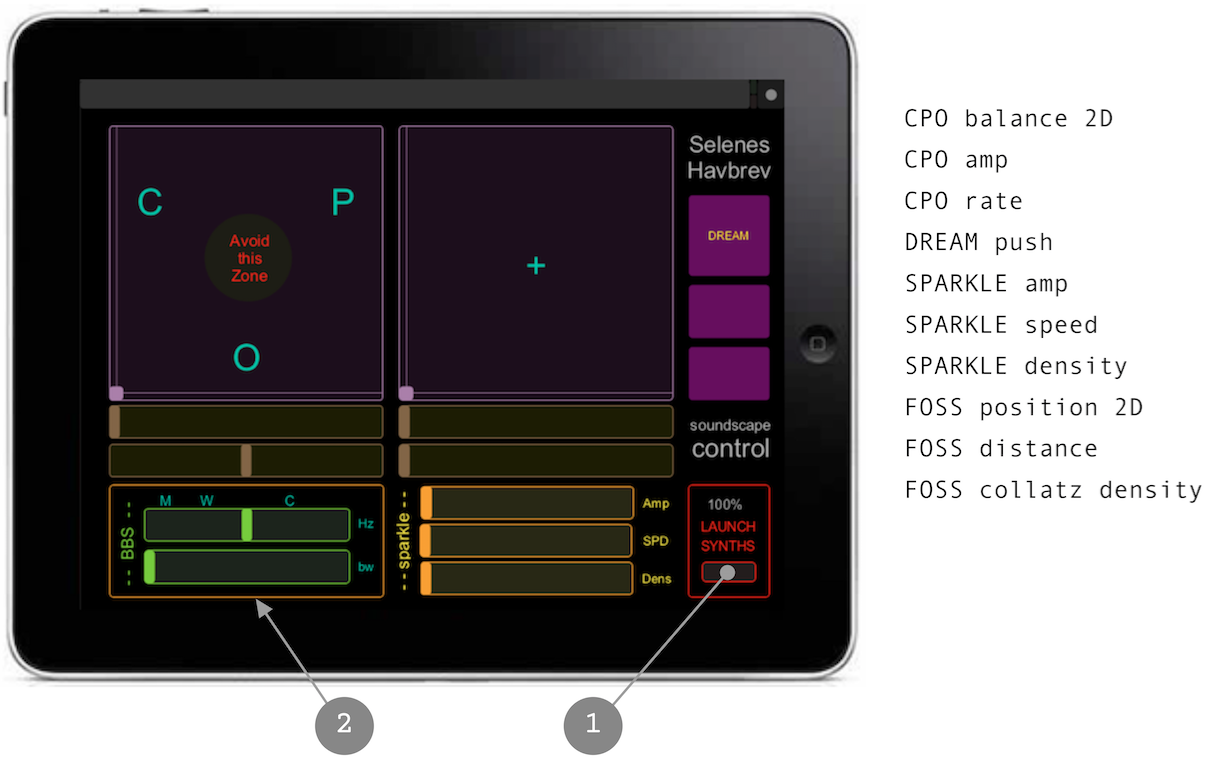
\includegraphics[width=0.87\textwidth]{mp/img/ipad2}
\end{figure}
\vspace{-5mm}
Layout used during the play on the 10th of October 2020 at Troms\o{} Kunstforening.
\end{enumerate}
\end{description}

On \textcolor{gray}{\large{\ding{202}}} stop and start the system -- boot SC plus start synths --, and on \textcolor{gray}{\large{\ding{203}}} a band reject filter applied to the soundscape according to the actor voices during the play.

\bigskip

\begin{description}
\item[Appendices] \hfill 
\begin{itemize}
\item[$\rightarrow$] Study with vibrating speakers on two recycled corrugated sheets as installation. This installation performed the score of the second guitar of the composition \textsl{Selenes Havbrev} as a MDS -- \textsl{\nameref{mds}} -- with the digital wave guide physical model of a bowed instrument (SuperCollider \textsl{Ugen} \texttt{DWGBowedSimple} part of the SC3plugins) and \texttt{RM236}.\\
\begin{figure}[H]
\hfill 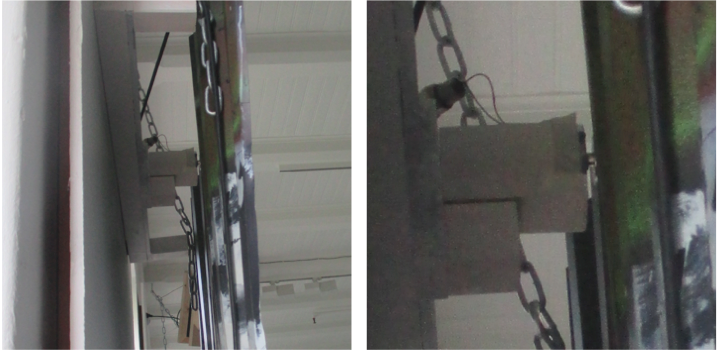
\includegraphics[width=0.87\textwidth]{mp/img/vs1a}
\end{figure}

\item[$\rightarrow$] Surrealistic sound installation experimenting the SuperCollider \textsl{Ugens} \texttt{DWGBowedSimple} -- playing with the bow parameters such as velocity, force and position --  and \texttt{NTube} (see Acoustics of Tube Models on page \pageref{atm}) -- playing alternatively with the input as a pink noise on two tubes and with the impulse oscillator on ten tubes -- (both are part of the SC3plugins) using respectively vibrating speakers on a cello and on a parabolic antenna, as part of a `post-apocalyptic' ambient quadraphonic soundscape.\\
\begin{figure}[H]
\hfill 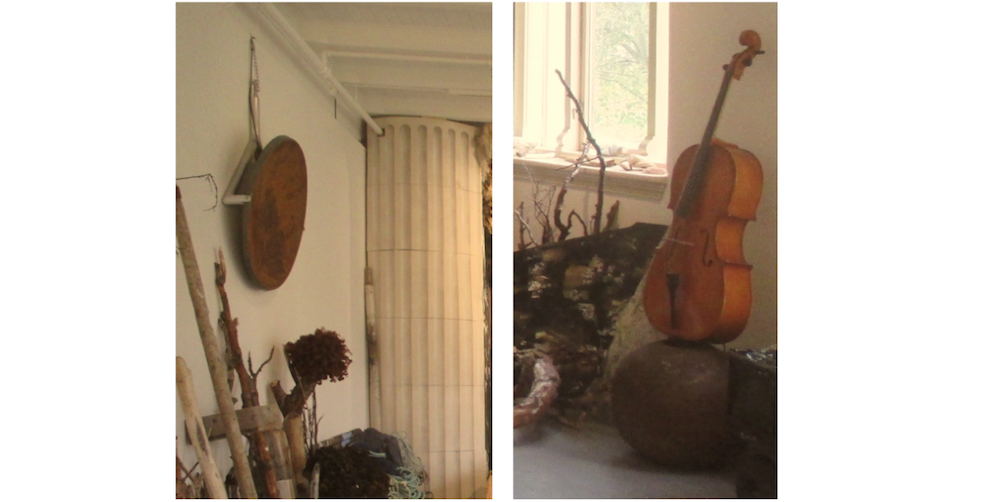
\includegraphics[width=0.87\textwidth]{mp/img/asc}
\end{figure}

\end{itemize}
\end{description}

%\bigskip

%\begin{center}\rule{0.5\linewidth}{0.5pt}\end{center}

%\bigskip


%% + works:  studies: study1 and study2

%\section*{Solutions}
%\phantomsection
%
%\addcontentsline{toc}{section}{Solutions}
%
%\bigskip
%
%\begin{description}
%\item[Concept] \hfill 
%\begin{itemize}
%\item[] ...
%\end{itemize}
%\bigskip
%\item[Context] \hfill 
%\begin{itemize}
%\item[] ...
%\end{itemize}
%\bigskip
%\bigskip
%\item[Source] \hfill 
%\begin{itemize}
%\item[] $\rightarrow$ \href{https://github.com/yannics/GSA/SC/Solutions.scd}{\texttt{\small https://github.com/yannics/GSA/SC/Solutions.scd}} 
%\end{itemize}
%\end{description}
%
%\bigskip
%
%\begin{center}\rule{0.5\linewidth}{0.5pt}\end{center}
%
%\bigskip
